
\documentclass{exam}

\usepackage{units} 
\usepackage{graphicx}
\usepackage[fleqn]{amsmath}
\usepackage{cancel}
\usepackage{float}
\usepackage{mdwlist}
\usepackage{booktabs}
\usepackage{cancel}
\usepackage{polynom}
\usepackage{caption}
\usepackage{fullpage}
\usepackage{xfrac}
\usepackage{enumerate}

\newcommand{\degree}{\ensuremath{^\circ}} 
\everymath{\displaystyle}

% \begin{figure}[H]
%   \centering
%   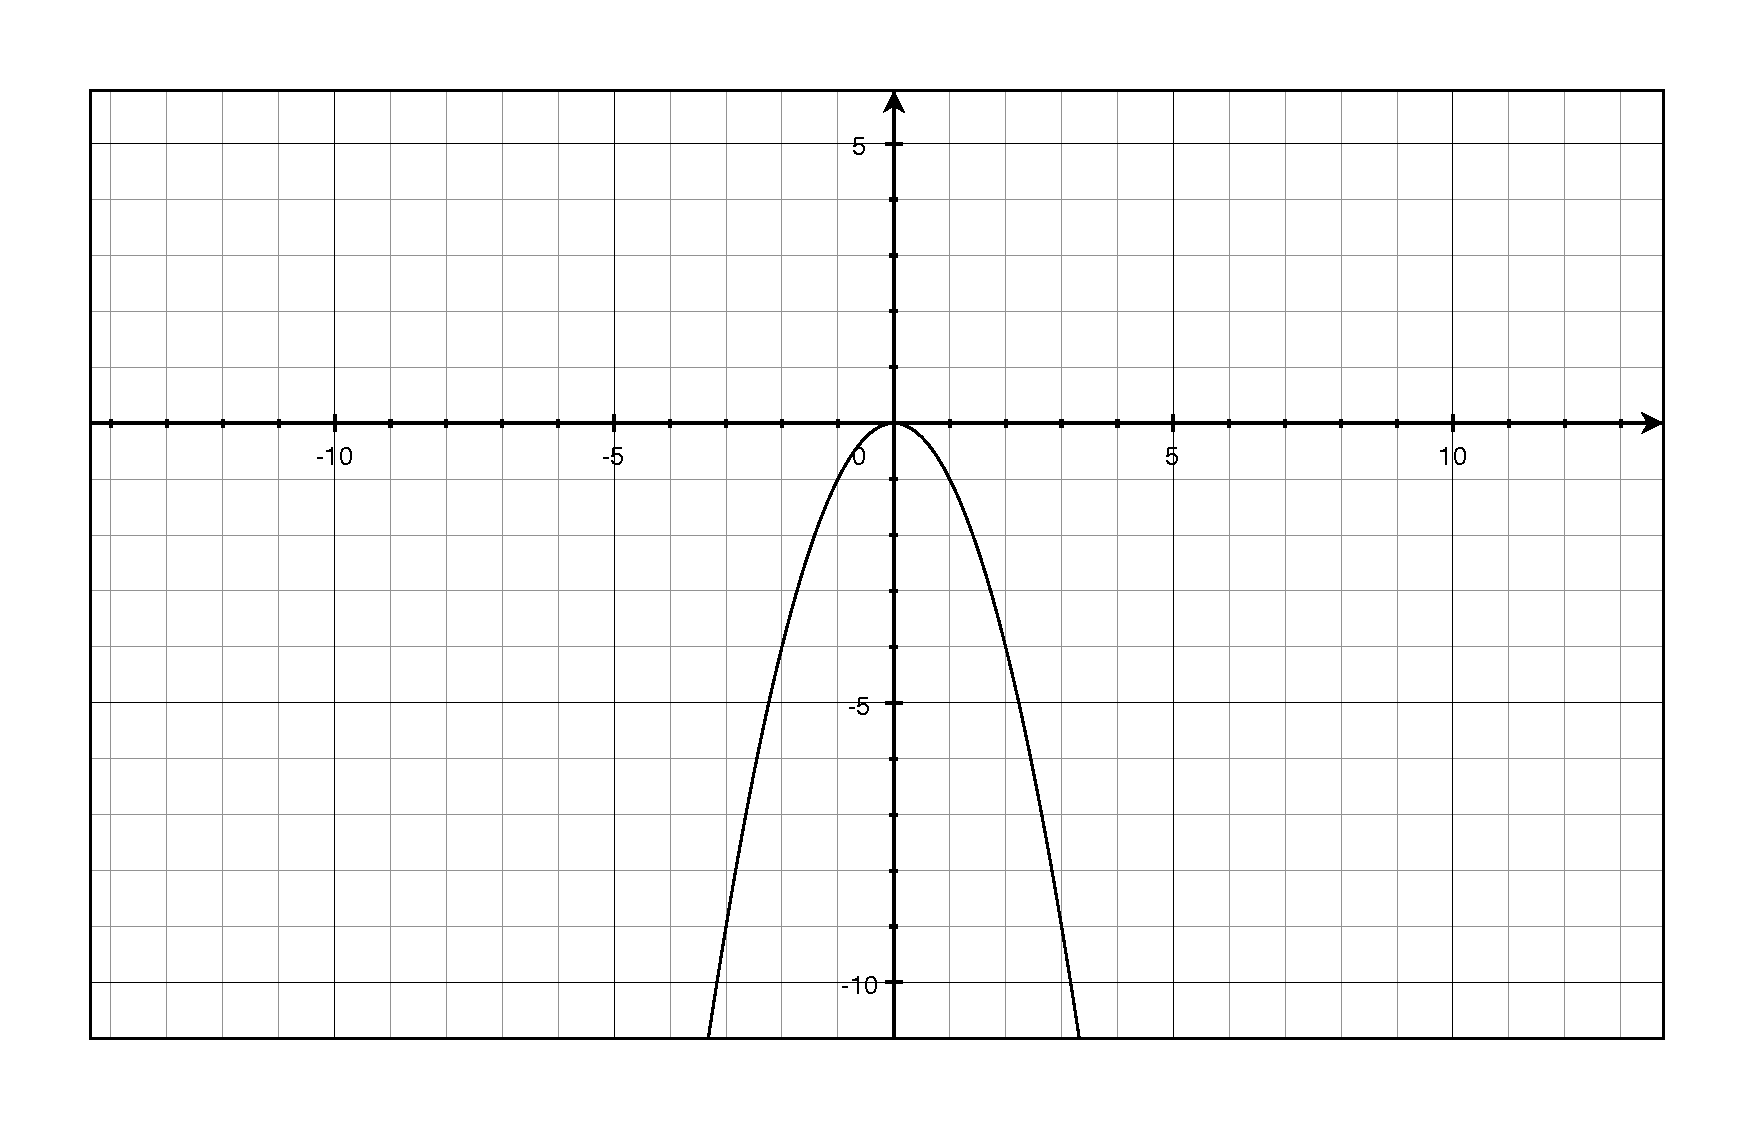
\includegraphics[scale=.3]{problem7.eps}
%   \caption*{Problem 7}
% \end{figure}

% \begin{tabular}{cc}
% \toprule
% period & amplitude \\
% \midrule
% value one & value two
% \bottomrule
% \end{tabular}

% \printanswers

\ifprintanswers 
  \usepackage{2in1, lscape} 
\fi

\date{May 1, 2013}
\author{}
\title{Math 141 \\ Homework 11}

\begin{document}

  \maketitle

  \section{Administrative}
  No class next week (5/8)

  \section{Homework}

  \begin{itemize*}
    \item Read Section 3.5 
    \item Section 3.5: 1-10, 15-19, 26-36, 38-39, 41-45, 49-54, 61-62, 64
  \end{itemize*}

  \section{Extra Credit}
  Section 3.5: 66-68

  \ifprintanswers
    \pagebreak

    \begin{description}
      \item[66]
        \begin{enumerate}[a]

          \item 
            \begin{align*}
              2x + 4i &= 1 \\
              x       &= \boxed{\frac{1}{2} - 2i} \\
            \end{align*}

          \item 
            \begin{align*}
              x^2 - ix &= 0 \\
              x(x - i) &= 0 \\
              x        &= \boxed{\left\{ 0, i \right\}} \\
            \end{align*}

          \item 
            \begin{align*}
              x^2 + 2ix - 1 &= 0 \\
              (x + i)^2     &= 0 \\
              x             &= \boxed{-i} \\
            \end{align*}

          \item 
            \begin{align*}
              ix^2 - 2x + i &= 0 \\
              \\
              x &= \frac{2 \pm \sqrt{4 - 4(i^2)}}{2i} \\
                &= \frac{2 \pm \sqrt{8}}{2i} \\
                &= \frac{1 \pm \sqrt{2}}{i} \left( \frac{i}{i} \right) \\
                &= \frac{i \pm i \sqrt{2}}{-1} \\
                &= \boxed{- i \left( 1 \pm \sqrt{2} \right)} \\
            \end{align*}
        \end{enumerate}

    \pagebreak

      \item[67]
        \[ f(x) = x^2 - (1 + i)x + (2 + 2i) \]

        \begin{enumerate}[a]
          \item 
            \begin{align*}
              f(2i) &= (2i)^2 - (1 + i)2i + (2 + 2i) \\
                    &= -4 - (2i - 2) + (2 + 2i) \\
                    &= -4 - 2i + 2 + 2 + 2i \\
                    &= 0 \\
              \\
              f(-2i) &= (-2i)^2 - (1 + i)(-2i) + (2 + 2i) \\
                     &= -4 + (2i + 2i^2) + (2 + 2i) \\
                     &= -4 + 2i - 2 + 2 + 2i \\
                     &= -4 + 4i \\
              \\
              f(1 - i) &= (1 - i)^2 - (1 + i)(1 - i) + (2 + 2i) \\
                       &= (1 - 2i + i^2) - (1 - i^2) + (2 + 2i) \\
                       &= - 2i - 2 + 2 + 2i \\
                       &= 0 \\
                       \\
              f(1 + i) &= (1 + i)^2 - (1 + i)(1 + i) + (2 + 2i) \\
                       &= (1 + i)^2 - (1 + i)^2 + (2 + 2i) \\
                       &= 2 + 2i \\
            \end{align*}

          \item The {\em Conjugate Zeros Theorem} only applies to functions with real coefficiencts.

        \end{enumerate}

    \pagebreak

      \item[68]
        \begin{enumerate}[a]
          \item 
            \begin{align*}
              f(x) &= (x - i)(x + i)(x - (1 + i))(x - (1 - i)) \\
                   &= (x^2 + 1)(x^2 - (1 +i)x - (1 - i)x + 2) \\
                   &= (x^2 + 1)(x^2 - 2x + 2) \\
                   &= \boxed{x^4 - 2x^3 + 3x^2 - 2x + 2} \\
            \end{align*}

          \item
            \begin{align*}
              f(x) &= (x - i)(x - (1 + i)) \\
                   &= x^2 - x(1 + i) -xi + i(1 + i) \\
                   &= x^2 - x - xi - xi + i + i^2 \\
                   &= \boxed{x^2 - (1 + 2i)x - (1 - i)} \\
            \end{align*}
        \end{enumerate}

    \end{description}

    \pagebreak

  \fi
  
  \section{Review}

  \begin{questions}
    \question Find two positive real numbers whose product is a maximum and the sum of the first and twice the second 
      is 24.

      \begin{solution}
        If $x$ and $y$ are the two numbers:
        \begin{align*}
          y + 2x &= 24 \\
          y      &= 24 - 2x \\
        \end{align*}

        We need to maximize:
        \begin{align*}
          f(x) &= xy \\
          &= x(24 - 2x) \\
          &= -2x^2 + 24x \\
        \end{align*}

        Find the maximum:
        \begin{align*}
          x  &= \frac{-b}{2a} \\
             &= \frac{-24}{-4} \\
             &= 6
          \\
          y  &= 24 - 12 \\
             &= 12 \\
        \end{align*}

        \fbox{The two numbers are 6 and 12}

      \end{solution}

    \question
      A broomstick manufacturer has daily production costs of:
      \[
        C(x) = 800 - 10x + 0.25x^2
      \]

      where $C$ is the total cost and $x$ is the number of broomsticks produced.  How many broomsticks should be
      produced each day to yield a minimum cost?

      \begin{solution}
        \begin{align*}
          x     &= \frac{10}{2 \cdot 0.25} \\
                &= 20 \\
          \\
          f(20) &= 700 \\
        \end{align*}

        \fbox{Producing 20 broomsticks each day minimizes costs.}

      \end{solution}

      \question 
        \[
          f(x) = \sqrt[3]{\frac{x + 1}{x^3 - 8}}
        \]

        What is the domain of $f$?

        \begin{solution}
          Since negative cube roots are fine, the only potential problem is a zero in the denominator.  This happens
          when:
          \begin{align*}
            x^3 - 8 &= 0 \\
            x &= \sqrt[3]{8} \\
            &= 2 \\
          \end{align*}

          So the domain is $\boxed{(\infty, 2) \cup (2, \infty)}$

        \end{solution}

  \end{questions}

  \ifprintanswers

    \section{Section 3.5}

    \begin{description}

      \item[1] 
        \begin{align*}
          P(x) &= x^4 + 4x^2 \\
               &= x^2(x^2 + 4) \\
               &= x^2(x + 2i)(x - 2i) \\
               \\
          x    &= \boxed{\left\{ 0, \pm 2i \right\}} \\
        \end{align*}

      \item[2] 
        \begin{align*}
          P(x) &= x^5 + 9x^3 \\
               &= x^3(x^2 + 9) \\
               &= x^3(x + 3i)(x - 3i) \\
               \\
          x    &= \boxed{\left\{ 0, \pm 3i \right\}} \\
        \end{align*}

      \item[3] 
        \begin{align*}
          P(x) &= x^3 - 2x^2 + 2x \\
               &= x(x^2 - 2x + 2) \\
               &= x(x - 1 + i))(x - 1 - i) \\
               \\
          x    &= \boxed{\left\{ 0, 1 \pm i \right\}} \\
        \end{align*}

      \item[4] 
        \begin{align*}
          P(x) &= x^3 + x^2 + x \\
               &= x(x^2 + x + 1) \\
               &= x \left(x + \frac{1}{2} - \frac{i \sqrt{3}}{2} \right) 
                  \left(x + \frac{1}{2} + \frac{i \sqrt{3}}{2} \right) \\
               \\
          x    &= \boxed{\left\{ 0, -\frac{1}{2} \pm \frac{i \sqrt{3}}{2} \right\}} \\
        \end{align*}

      \item[5] 
        \begin{align*}
          P(x) &= x^4 + 2x^2 + 1 \\
               &= (x^2 + 1)^2 \\
               &= (x + i)^2(x - i)^2 \\
               \\
          x    &= \boxed{\left\{ \pm i \right\}} \\
        \end{align*}

      \item[6] 
        \begin{align*}
          P(x) &= x^4 - x^2 - 2 \\
               &= \left(x^2-2\right) \left(x^2+1\right) \\
               &= (x + \sqrt{2}) (x - \sqrt{2}) (x + i) (x - i) \\
               \\
          x    &= \boxed{\left\{ \pm \sqrt{2}, \pm i \right\}} \\
        \end{align*}

      \item[7] 
        \begin{align*}
          P(x) &= x^4 - 16 \\
               &= (x^2 + 4)(x^2 - 4) \\
               &= (x + 2i)(x - 2i)(x + 2)(x - 2) \\
               \\
          x    &= \boxed{\left\{ \pm 2, \pm 2i \right\}} \\
        \end{align*}

      \item[8] 
        \begin{align*}
          P(x) &= x^4 + 6x^2 + 9 \\
               &= (x^2 + 3)^2 \\
               &= (x + i \sqrt{3})^2(x - i \sqrt{3})^2 \\
               \\
          x    &= \boxed{\left\{ \pm i \sqrt{3} \right\}} \\
        \end{align*}

      \item[9] 
        \begin{align*}
          P(x) &= x^3 + 8 \\
               &= (x+2) \left(x^2-2 x+4\right) \\
               &= (x + 2)(x - 1 - i \sqrt{3})(x - 1 + i \sqrt{3}) \\
               \\
          x    &= \boxed{\left\{ -2, 1 \pm i \sqrt{3} \right\}} \\
        \end{align*}

      \item[10] 
        \begin{align*}
          P(x) &= x^3 - 8 \\
               &= (x - 2)(x^2 + 2x + 4) \\
               &= (x - 2)(x + 1 - i \sqrt{3})(x + 1 + i \sqrt{3}) \\
               \\
          x    &= \boxed{\left\{ 2, -1 \pm i \sqrt{3} \right\}} \\
        \end{align*}

      \item[15] 
        \begin{align*}
          P(x) &= x^2 + 2x + 2 \\
               &= (x + 1 + i)(x + 1 - i) \\
               \\
          x    &= \boxed{\left\{ -1 \pm i \right\}} \\
        \end{align*}

      \item[16] 
        \begin{align*}
          P(x) &= x^2 - 8x + 17 \\
               &= (x - 4 + i)(x - 4 - i) \\
               \\
          x    &= \boxed{\left\{ 4 \pm i \right\}} \\
        \end{align*}

      \item[17] 
        \begin{align*}
          P(x) &= x^3 + 4x \\
               &= x(x^2 + 4) \\
               &= x(x + 2i)(x - 2i) \\
               \\
          x    &= \boxed{\left\{ 0, \pm 2i \right\}} \\
        \end{align*}

      \item[18] 
        \begin{align*}
          P(x) &= x^3 - x^2 + x \\
               &= x(x^2 - x + 1) \\
               &= x(x - \frac{1}{2}+\frac{i \sqrt{3}}{2})(x - \frac{1}{2}-\frac{i \sqrt{3}}{2})
               \\
          x    &= \boxed{\left\{ 0, \frac{1}{2} \pm \frac{i \sqrt{3}}{2} \right\}} \\
        \end{align*}

      \item[19] 
        \begin{align*}
          P(x) &= x^4 - 1 \\
               &= (x^2 - 1)(x^2 + 1) \\
               &= (x + 1)(x - 1)(x + i)(x - i) \\
               \\
          x    &= \boxed{\left\{ \pm 1, \pm i \right\}} \\
        \end{align*}

      \item[26] 
        \begin{align*}
          P(x) &= x^4 + 10x^2 + 25 \\
               &= (x^2 + 5)^2 \\
               &= (x + i \sqrt{5})^2(x - i \sqrt{5})^2  \\
               \\
          x    &= \boxed{\left\{ \pm i \sqrt{5} \right\}} \\
        \end{align*}

        Both zeros have multiplicity 2.

      \item[27] 
        \begin{align*}
          P(x) &= x^4 + 3x^2 - 4 \\
               &= (x^2 - 1)(x^2 + 4) \\
               &= (x + 1)(x - 1)(x + 2i)(x - 2i) \\
               \\
          x    &= \boxed{\left\{ \pm 1, \pm 2i \right\}} \\
        \end{align*}

      \item[28] 
        \begin{align*}
          P(x) &= x^5 + 7x^3 \\
               &= x^3(x^2 + 7) \\
               &= x^3(x + i \sqrt{7})(x - i \sqrt{7}) \\
               \\
          x    &= \boxed{\left\{ 0, \pm i \sqrt{7} \right\}} \\
        \end{align*}

        0 has multiplicity 3

      \item[29] 
        \begin{align*}
          P(x) &= x^5 + 6x^3 + 9x \\
               &= x(x^4 + 6x^2 + 9) \\
               &= x(x^2 + 3)^2 \\
               &= x(x + i \sqrt{3})^2(x - i \sqrt{3})^2 \\
               \\
          x    &= \boxed{\left\{ 0, \pm i \sqrt{3} \right\}} \\
        \end{align*}

        $\pm i \sqrt{3}$ has a multiplicity of 2

      \item[30] 
        \begin{align*}
          P(x) &= x^6 + 16x^3 + 64 \\
               &= (x^3 + 8)^2 \\
               &= \left[ (x + 2)(x^2 - 2x + 4) \right]^2 \\
               &= \left[ (x + 2)(x - 1 - i \sqrt{3})(x - 1 + i \sqrt{3}) \right]^2 \\
               \\
          x    &= \boxed{\left\{ -2, 1 \pm i \sqrt{3} \right\}} \\
        \end{align*}

        All zeros have a multiplicity of 2.

      \item[31]
        \begin{align*}
          P(x) &= (x - (1 + i)) (x - (1 - i)) \\
               &= \boxed{x^2 - 2x + 2} \\
        \end{align*}

      \item[32]
        \begin{align*}
          P(x) &= (x - (1 + i \sqrt{2})) (x - (1 - i \sqrt{2})) \\
               &= \boxed{x^2 - 2x + 3} \\
        \end{align*}

      \item[33]
        \begin{align*}
          P(x) &= (x - 3) (x - 2i) (x + 2i) \\
               &= (x - 3) (x^2 + 4)\\
               &= \boxed{x^3 - 3x^2 + 4x - 12} \\
        \end{align*}

      \item[34]
        \begin{align*}
          P(x) &= x (x - i) (x + i) \\
               &= x (x^2 + 1) \\
               &= \boxed{x^3 + x} \\
        \end{align*}

      \item[35]
        \begin{align*}
          P(x) &= (x - 2) (x - i) (x + i) \\
               &= (x - 2) (x^2 + 1) \\
               &= \boxed{x^3 - 2x^2 + x - 2} \\
        \end{align*}

      \item[36]
        \begin{align*}
          P(x) &= (x + 3) (x - (1 + i)) (x + (1 - i)) \\
               &= \boxed{x^3 + x^2 - 4x + 6} \\
        \end{align*}

      \item[38]
        \begin{align*}
          P(x) &= (x + 2i)(x - 2i)(x + 3i)(x - 3i) \\
               &= (x^2 + 4)(x^2 + 9) \\
               &= \boxed{x^4 + 13x^2 + 36} \\
        \end{align*}

      \item[39]
        First find a function with the correct zeros:
        \begin{align*}
          P(x) &= (x + i) (x - i) (x - (i + 1)) (x - (-i + 1)) \\
               &= (x^2 + 1)(x^2 - 2x + 2) \\
               &= x^4 - 2x^3 + 3x^2 - 2x + 2 \\
        \end{align*}

        Multiply by 6 to get a constant term of 12:
        \[
           \boxed{P(x) = 6x^4 - 12x^3 + 18x^2 - 12x + 12} \\
        \]
      \item[41]
        \begin{align*}
          P(x) &= x^3 + 2x^2 + 4x + 8 \\
               &= x^2(x + 2) + 4(x + 2) \\
               &= (x^2 + 4)(x + 2) \\
               \\
          x    &= \boxed{\left\{ -2, \pm 2i \right\}} \\
        \end{align*}

      \item[42]
        \begin{align*}
          P(x) &= x^3 - 7x^2 + 17x - 15 \\
               &= (x - 3) (x^2 - 4x + 5) \\
               \\
          x    &= \boxed{\left\{ 3, 2 \pm i \right\}} \\
        \end{align*}

      \item[43]
        \begin{align*}
          P(x) &= x^3 - 2x^2 + 2x - 1 \\
               &= (x-1) \left( x^2-x+1 \right) \\
               \\
          x    &= \boxed{\left\{ 1, \frac{1}{2} \pm \frac{i \sqrt{3}}{2} \right\}} \\
        \end{align*}

      \item[44]
        \begin{align*}
          P(x) &= x^3 + 7x^2 + 18x + 18 \\
               &= (x+3) (x^2 + 4x + 6) \\
               \\
          x    &= \boxed{\left\{ -3, -2 \pm i \sqrt{2} \right\}} \\
        \end{align*}

      \item[45]
        \begin{align*}
          P(x) &= x^3 - 3x^2 + 3x - 2 \\
               &= (x-2)(x^2 - x + 1) \\
               \\
          x    &= \boxed{\left\{ 2, \frac{1}{2} \pm \frac{i \sqrt{3}}{2} \right\}} \\
        \end{align*}

      \item[49]
        \begin{align*}
          P(x) &= x^4 + x^3 + 7x^2 + 9x - 18 \\
               &= (x-1) (x+2) (x^2 + 9) \\
               \\
          x    &= \boxed{\left\{ -2, 1, \pm 3i \right\}} \\
        \end{align*}

      \item[50]
        \begin{align*}
          P(x) &= x^4 - 2x^3 - 2x^2 - 2x - 3 \\
               &= (x-3) (x+1) \left( x^2 + 1 \right) \\
               \\
          x    &= \boxed{\left\{ 3, -1, \pm i \right\}} \\
        \end{align*}

      \item[51]
        \begin{align*}
          P(x) &= x^5 - x^4 + 7x^3 - 7x^2 + 12x - 12 \\
               &= (x - 1) \left( x^4 + 7x^2 + 12 \right) \\
               &= (x - 1) \left(x^2 + 3\right) \left(x^2 + 4\right) \\
               \\
          x    &= \boxed{\left\{ 1, \pm i \sqrt{3}, \pm 2i \right\}} \\
        \end{align*}

      \item[52]
        \begin{align*}
          P(x) &= x^5 + x^3 + 8x^2 + 8 \\
               &= x^3(x^2 + 1) + 8(x^2 + 1) \\
               &= \left( x^2 + 1 \right)\left( x^3 + 8 \right) \\
               &=  \left(x^2 + 1\right) (x + 2) \left(x^2 - 2x + 4\right) \\
               \\
          x    &= \boxed{\left\{ -2, \pm i, 1 \pm i \sqrt{3} \right\}} \\
        \end{align*}

      \item[53]
        \begin{align*}
          P(x) &= x^4 - 6x^3 + 13x^2 - 24x + 36 \\
               &= (x - 3)^2 \left(x^2 + 4\right) \\
               \\
          x    &= \boxed{\left\{ 3, \pm 2i \right\}} \\
        \end{align*}

      \item[54]
        \begin{align*}
          P(x)    &= x^4 - x^2 + 2x + 2 \\
                  &= (x + 1) \left( x^3 - x^2 + 2 \right) \\
                  &= (x + 1)^2 \left(x^2 - 2x + 2\right) \\
               \\
          x       &= \boxed{\left\{ -1, 1 \pm i \right\}} \\
        \end{align*}

  %     \item[60]
  %       \begin{align*}
  %         P(x) &= x^3 - 2x - 4 \\
  %              &= (x-2) \left(x^2+2 x+2\right) \\
  %              &= (x-2) (x + 1 + i) (x + 1 - i) \\
  %       \end{align*}

      \item[61]
        \begin{align*}
          P(x) &= x^4 + 8x^2 - 9 \\
               &= \left( x^2 + 9 \right) \left( x^2 - 1 \right) \\
               &= \left( x^2 + 9 \right) (x + 1) (x - 1) \\
               &= \boxed{(x + 3i) (x - 3i) (x + 1) (x - 1)} \\
        \end{align*}

      \item[62]
        \begin{align*}
          P(x) &= x^4 + 8x^2 + 16 \\
               &= \left( x^2 + 4 \right)^2 \\
               &= \boxed{(x + 2i)^2 (x - 2i)^2} \\
        \end{align*}

      \item[64]
        \begin{align*}
          P(x) &= x^5 - 16x \\
               &= x \left( x^4 - 16 \right) \\
               &= x \left( x^2 + 4 \right) \left( x^2 - 4 \right) \\
               &= \boxed{x (x + 2i) (x - 2i) (x + 2) (x - 2)} \\
        \end{align*}

  %     \item[63]
  %       \begin{align*}
  %         P(x) &= x^6 - 64 \\
  %              &= \left( x^3 - 8 \right)\left( x^3 + 8 \right) \\
  %              &= (x-2) \left(x^2+2 x+4\right) (x+2) \left(x^2-2 x+4\right)  \\
  %       \end{align*}

    \end{description}

  \else
    \vspace{1.5 cm}
    \begin{quote}
      \begin{em}
        Science is the belief in the ignorance of experts. 
      \end{em}
    \end{quote}

    \hspace{1 cm} --Richard Feynman


  \fi

\end{document}

